%% This is file `elsarticle-template-1-num.tex',
%%
%% Copyright 2009 Elsevier Ltd
%%
%% This file is part of the 'Elsarticle Bundle'.
%% ---------------------------------------------
%%
%% It may be distributed under the conditions of the LaTeX Project Public
%% License, either version 1.2 of this license or (at your option) any
%% later version.  The latest version of this license is in
%%    http://www.latex-project.org/lppl.txt
%% and version 1.2 or later is part of all distributions of LaTeX
%% version 1999/12/01 or later.
%%
%% The list of all files belonging to the 'Elsarticle Bundle' is
%% given in the file `manifest.txt'.
%%
%% Template article for Elsevier's document class `elsarticle'
%% with numbered style bibliographic references
%%
%% $Id: elsarticle-template-1-num.tex 149 2009-10-08 05:01:15Z rishi $
%% $URL: http://lenova.river-valley.com/svn/elsbst/trunk/elsarticle-template-1-num.tex $
%%
\documentclass[preprint,12pt]{elsarticle}

%% Use the option review to obtain double line spacing
%% \documentclass[preprint,review,12pt]{elsarticle}

%% Use the options 1p,twocolumn; 3p; 3p,twocolumn; 5p; or 5p,twocolumn
%% for a journal layout:
%% \documentclass[final,1p,times]{elsarticle}
%% \documentclass[final,1p,times,twocolumn]{elsarticle}
%% \documentclass[final,3p,times]{elsarticle}
%% \documentclass[final,3p,times,twocolumn]{elsarticle}
%% \documentclass[final,5p,times]{elsarticle}
%% \documentclass[final,5p,times,twocolumn]{elsarticle}

%% if you use PostScript figures in your article
%% use the graphics package for simple commands
%% \usepackage{graphics}
%% or use the graphicx package for more complicated commands
%% \usepackage{graphicx}
%% or use the epsfig package if you prefer to use the old commands
%% \usepackage{epsfig}

%% The amssymb package provides various useful mathematical symbols
\usepackage{amssymb}
%% The amsthm package provides extended theorem environments
%% \usepackage{amsthm}

%% The lineno packages adds line numbers. Start line numbering with
%% \begin{linenumbers}, end it with \end{linenumbers}. Or switch it on
%% for the whole article with \linenumbers after \end{frontmatter}.
\usepackage{lineno}

%% natbib.sty is loaded by default. However, natbib options can be
%% provided with \biboptions{...} command. Following options are
%% valid:

%%   round  -  round parentheses are used (default)
%%   square -  square brackets are used   [option]
%%   curly  -  curly braces are used      {option}
%%   angle  -  angle brackets are used    <option>
%%   semicolon  -  multiple citations separated by semi-colon
%%   colon  - same as semicolon, an earlier confusion
%%   comma  -  separated by comma
%%   numbers-  selects numerical citations
%%   super  -  numerical citations as superscripts
%%   sort   -  sorts multiple citations according to order in ref. list
%%   sort&compress   -  like sort, but also compresses numerical citations
%%   compress - compresses without sorting
%%
%% \biboptions{comma,round}

% \biboptions{}


\journal{NIM A}

\begin{document}



\begin{frontmatter}

%% Title, authors and addresses

%% use the tnoteref command within \title for footnotes;
%% use the tnotetext command for the associated footnote;
%% use the fnref command within \author or \address for footnotes;
%% use the fntext command for the associated footnote;
%% use the corref command within \author for corresponding author footnotes;
%% use the cortext command for the associated footnote;
%% use the ead command for the email address,
%% and the form \ead[url] for the home page:
%%
%% \title{Title\tnoteref{label1}}
%% \tnotetext[label1]{}


%% \ead[url]{home page}
%% \fntext[label2]{}

%% \address{Address\fnref{label3}}
%%\fntext[label3]{dfd}

\title{Performance of Water-based Liquid Scintillator}

%% use optional labels to link authors explicitly to addresses:
%% \author[label1,label2]{<author name>}
%% \address[label1]{<address>}
%% \address[label2]{<address>}
 \author[label1]{D. Beznosko\corref{cor1}}
 \ead{dima@dozory.us}
%%\cortext[cor1]{4107 47ave, 3D, Sunnyside, NY 11104}
\author[label2]{M.V. Diwan}
\author[label3]{S.Hans}
\author[label2]{D. Jaffe}
\author[label2]{S.H. Kettell}
\author[label3]{R.Rosero}
\author[label2]{H. Themann}
\author[label2]{B. Viren}
\author[label2]{E. Worcester}
\author[label3]{M. Yeh}
\author[label2]{C. Zhang}
\address[label2]{Physics Department, Brookhaven National Laboratory, Upton, NY 11973, USA }
\address[label3]{Chemistry Department, Brookhaven National Laboratory, Upton, NY 11973, USA }
\address[label1]{Department of Physics, Nazarbayev University, Astana, 010000, KZ }





\begin{abstract}

	The Water-based Liquid Scintillator (WbLS) is a new material currently under development. It is based on the idea of dissolving the organic scintillator in water using special surfactants. This material strives to achieve the novel detection techniques by combining the Cerenkov rings and scintillation light, as well as the total cost reduction compared to pure liquid scintillator (LS).

	Presented are the light yield measurements for the three different proton beam energies (210MeV, 475MeV and 2000MeV) for water, two different WbLS formulations (0.4$\%$ and 0.99$\%$) and pure LS. The results show that a goal of ~100 optical photons/MeV, indicated by the simulation to be an optimal light yield for observing both the Cerenkov ring and scintillaton light from the proton decay in a large water detector, has been achieved.

\end{abstract}

\begin{keyword}
%% keywords here, in the form: keyword \sep keyword
Water based \sep liquid scintillator \sep beam test
%% MSC codes here, in the form: \MSC code \sep code
%% or \MSC[2008] code \sep code (2000 is the default)

\end{keyword}

\end{frontmatter}

%%
%% Start line numbering here if you want
%%
 \linenumbers

%% main text
\section{Motivation}
\label{introAndMotivation}
In large water detectors, the Cerenkov radiation produced by a charged particle above the threshold can be used for particle identification, and the reconstruction of its direction and energy~\cite{superKkinematik}. However, all charged particles below the Cherenkov threshold are missed. Detecting these below-threshold particles is important for various applications. For example, in the search of the proton decay, in the $p^{+} \rightarrow K^{+} \overline{\nu}$ channel, where K\textsuperscript{+} is mostly below Cerenkov threshold and is invisible is a water detector. The use of the WbLS makes the kaon visible and allows for the 
separation of K$^{+}$, $\mu^{+}$ and e\textsuperscript{+} signals using timing and reduce background for this decay channel.

In either LS or WbLS, the isotropic scintillation light is produced by the charged particle energy deposition via ionization, but the scintillator components may interfere with the Cerenkov ring detection. To detect K\textsuperscript{+} and preserve the Cerenkov ring, MC studies indicate that the light yield (LY) from the scintillator component int he WbLS should be ~100 optical photons/MeV.

Thus, WbLS potentially combines both the Cerenkov ring and scintillation light capabilities. It can preserve the particle identification for the particles above the Cerenkov threshold, and detect the charged particles below the threshold via the scintillation light. In addition, WbLS features the lower cost than pure LS and it is safer to handle[ask Minfang for reference].

The ability to reach the desired LY can be checked using the monoenergetic proton beam with different WbLS concentrations. For the test, the two different WbLS formulations (0.4$\%$ and 0.99$\%$), pure water and pure LS samples were chosen. Three different proton beam energies were used with each sample. The choice of the energies comes from the following considerations: 

\begin{itemize}
	\item 2000MeV protons behave as minimum ionizing particle (MIP)
	\item 475MeV protons are just below the Cerenkov limit in water
	\item 210MeV protons have $\sim$same energy deposition as K$^{+}$ from the proton decay channel mentioned above.
\end{itemize}
 


 \section{Experimental Setup}
 \label{setup1}

The experimental setup used for the proton beam test is shown in (Figure~\ref{experimentalsetup1}). Two tubs with the samples were used (T1 and T2). Three 2cm x 2cm 5mm thick plastic scintillator hodoscopes were used (H1 to H3) with the beam trigger being formed by the coincidence of the H1\&H2 only. H3 was intended to verify whether particles exit T2.
\begin{figure}[ht]
\centering
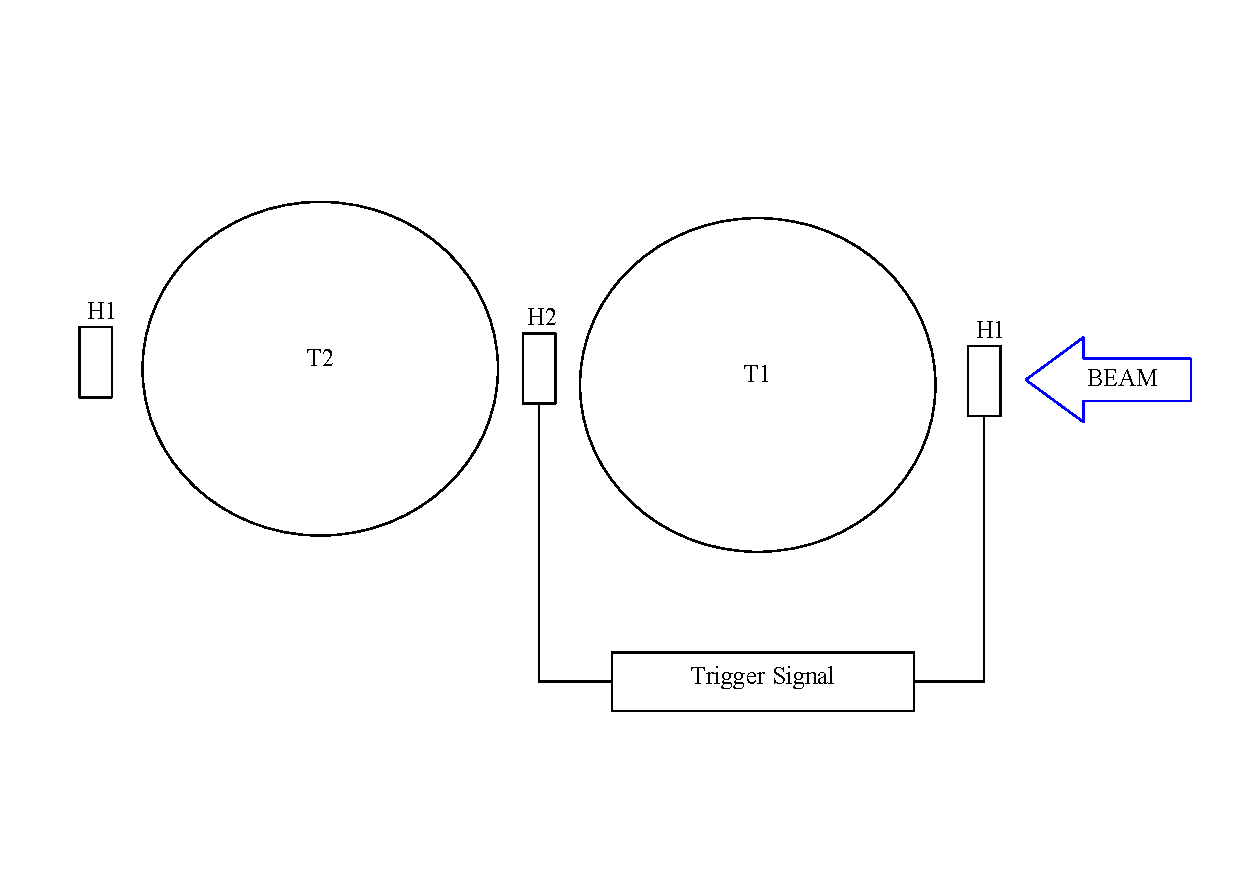
\includegraphics[width=100mm]{beamtestschematics1.pdf}
\caption{Proton beam test experimental setup.} \label{experimentalsetup1}
\end{figure}.





\subsection{Tub and Signal Readout Description}
\label{tubs}
Two tubs were used in the experiment:

\begin{itemize}
	\item T1 from Polytetrafluoroethylene (PTFE) (white, highly reflective),
  \item T2 from Aluminum, coated with black PTFE (very low reflectivity).
\end{itemize}

The T1 allows the capture of most of the light produced in the tub, whereas T2 allows for the observation of the light coming directly from the scintillation without the multiple wall reflections. An image of a tub is in (Figure~\ref{whitetubpicture}). Both T1 and T2 have the same dimensions:

\begin{itemize}
	\item the lid is 19.05mm thick,
	\item the walls and bottom are 6.35mm thick,
	\item inner height and diameter are 150mm.
\end{itemize}

\begin{figure}[ht]
\centering
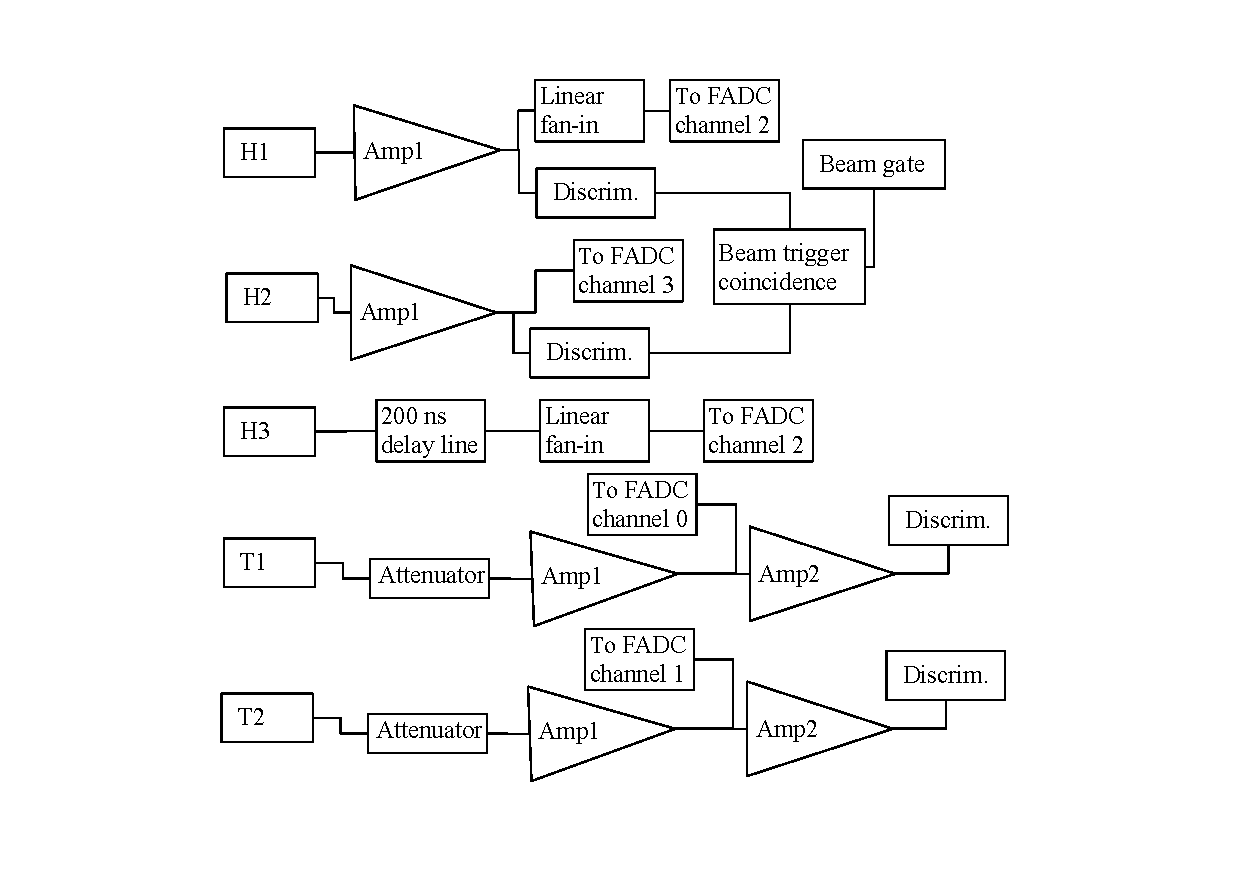
\includegraphics[width=130mm]{beamtestschematics.pdf}
\caption{Proton beam test experimental setup.} \label{experimentalsetup2}
\end{figure}.

A detailed setup readout scheme is shown in (Figure~\ref{experimentalsetup2}). Both tubs were read out by Hamamatsu~\cite{hamamatsu} R7723 2"  Photo-multiplier tubes (PMT). A readout was by the 4-channel 14bit CAEN~\cite{caen} V1729A Flash Analog-to-Digital Converter (FADC). All tubs signals were connected to the FADC via a variable attenuation unit (Phillips Scientific~\cite{phillips} 804) and a variable amplifier unit (Phillips Scientific 778). For the T1 and the T2 readouts, the gain was set to the values of $\sim$2x. The first output from the amplifier goes to the FADC, with a dedicated channel for each tub. The second output from each amplifier channel was used for the single ptoho-electron (PE) calibration. The gain for the second amplification stage was set at $\sim$10x.

All hodoscopes are also connected via $\sim$2x gain amplifier channels that allows signal splitting. H1 and H3 share the same FADC channel with latter signal being delayed by 200ns. H2 is connected to the last remaning channel of the FADC.





\begin{figure}[ht]
\centering
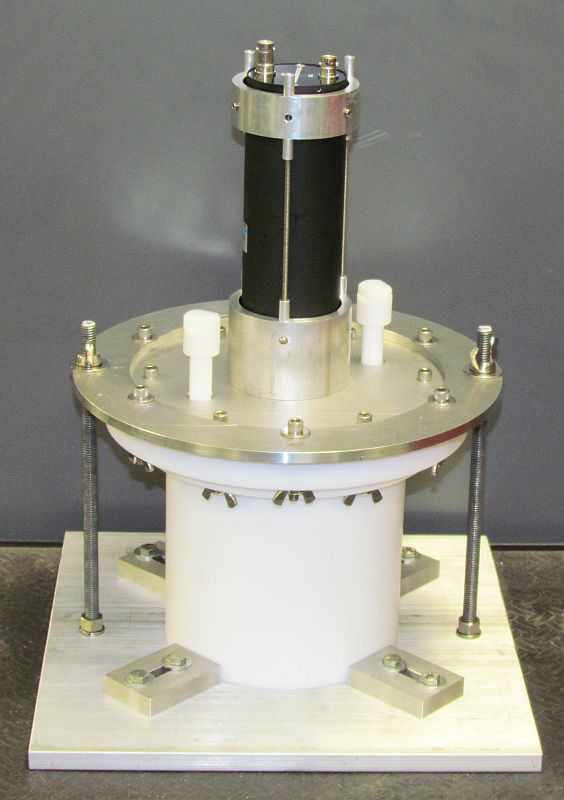
\includegraphics[width=50mm]{figure1_tub.jpg}
\caption{PTFE tub detector with a PMT.} \label{whitetubpicture}
\end{figure}

\subsection{Triggering Scheme}
\label{trigs}
Triggering schema was realized using three 2cm x 2cm, 5mm thick plastic scintillator counters that were readout by 2" PMTs via an air waveguide in order to remove the PMTs from direct beam exposure. The signal from the frontmost and a middle counters were used to form a bean trigger, as indicated in the (Figure~\ref{experimentalsetup2})




\subsection{Proton Beamline Description}
A proton test beam was conducted at NASA Space Radiation Laboratory (NSRL) facility at BNL. As described above, the three proton beam energies were used:
210MeV, 475MeV and 2GeV. The beam had the following main characteristics:

\begin{itemize}
	\item intensity of $\sim$1p+/bunch,
	\item beam size was ~1cm x1cm at 2GeV and 5.4cm x 5.4cm at 210MeV,
	\item 0.4s long spills every $\sim$4 sec.
\end{itemize}

%%%%%%%%%%%%%%%%%%%%%%%%%%%%%%%%%%%%%%%%%%%%%%%%%
 \section{Data Analysis}
\label{dataanalysis}
\subsection{Liquids Measured}


\subsection{Waveform Analysis}


\begin{figure}[ht]
\centering
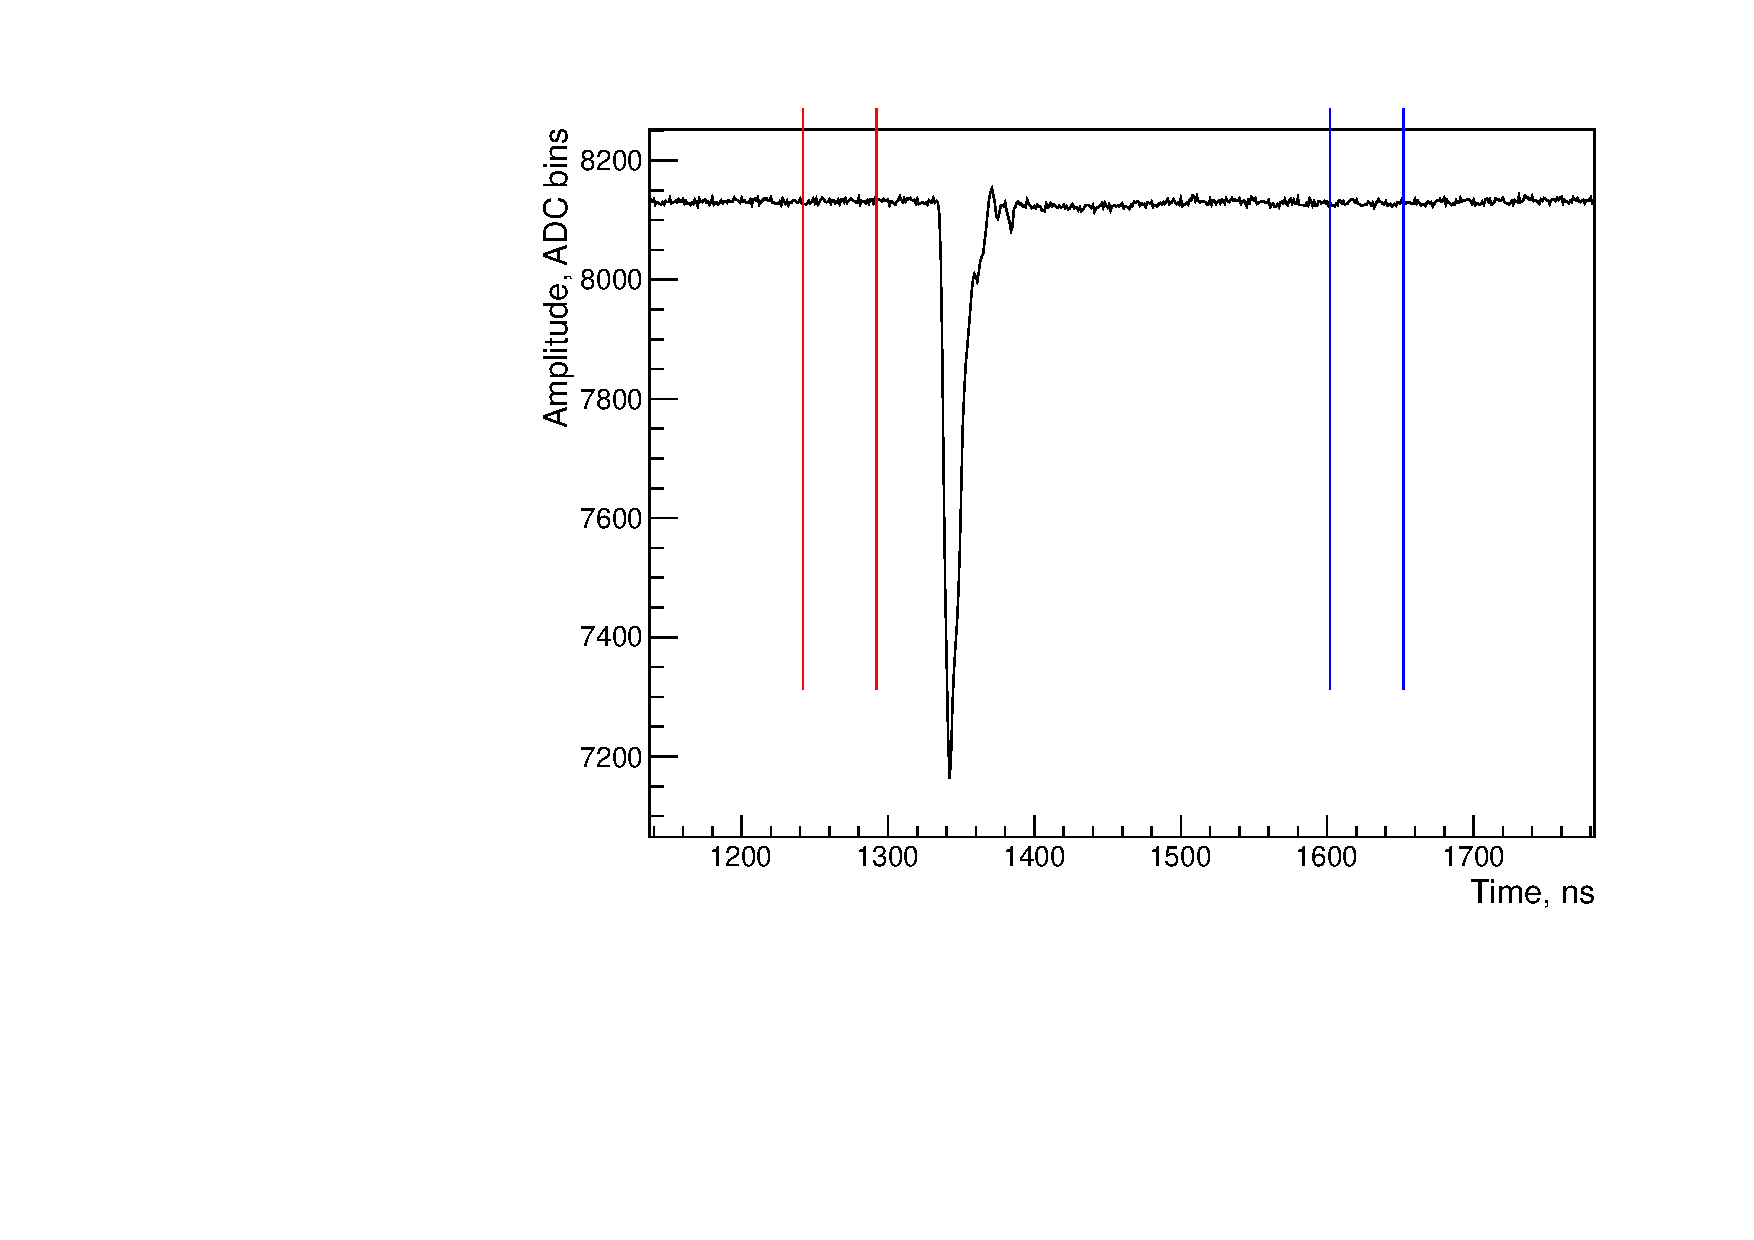
\includegraphics[width=80mm]{PMTtypicalSignal.pdf}
\caption{Typical PMT waveform with baseline check windows.} \label{typicalpmtsignal}
\end{figure}

The PMT signal is acquired as a waveform shown in (Figure~\ref{typicalpmtsignal}). Total aquisition window is 2560 bins per event with each bin being 1ns wide; the signal is approximately centered and the approximate position is known beforehand. A 300ns window (central one in the figure, between the red and blue lines) is used to obtain the integrated signal area by summation. Each point is subtracted from the average baseline to achieve a positive sum. A typical signal is smaller then the chosen window width, however, there is a small spread in timing of the signals and we want' to be sure that all of the signal has been integrated. The size of the chosen window is the same for all samples and measurememnts.

\begin{figure}[ht]
\centering
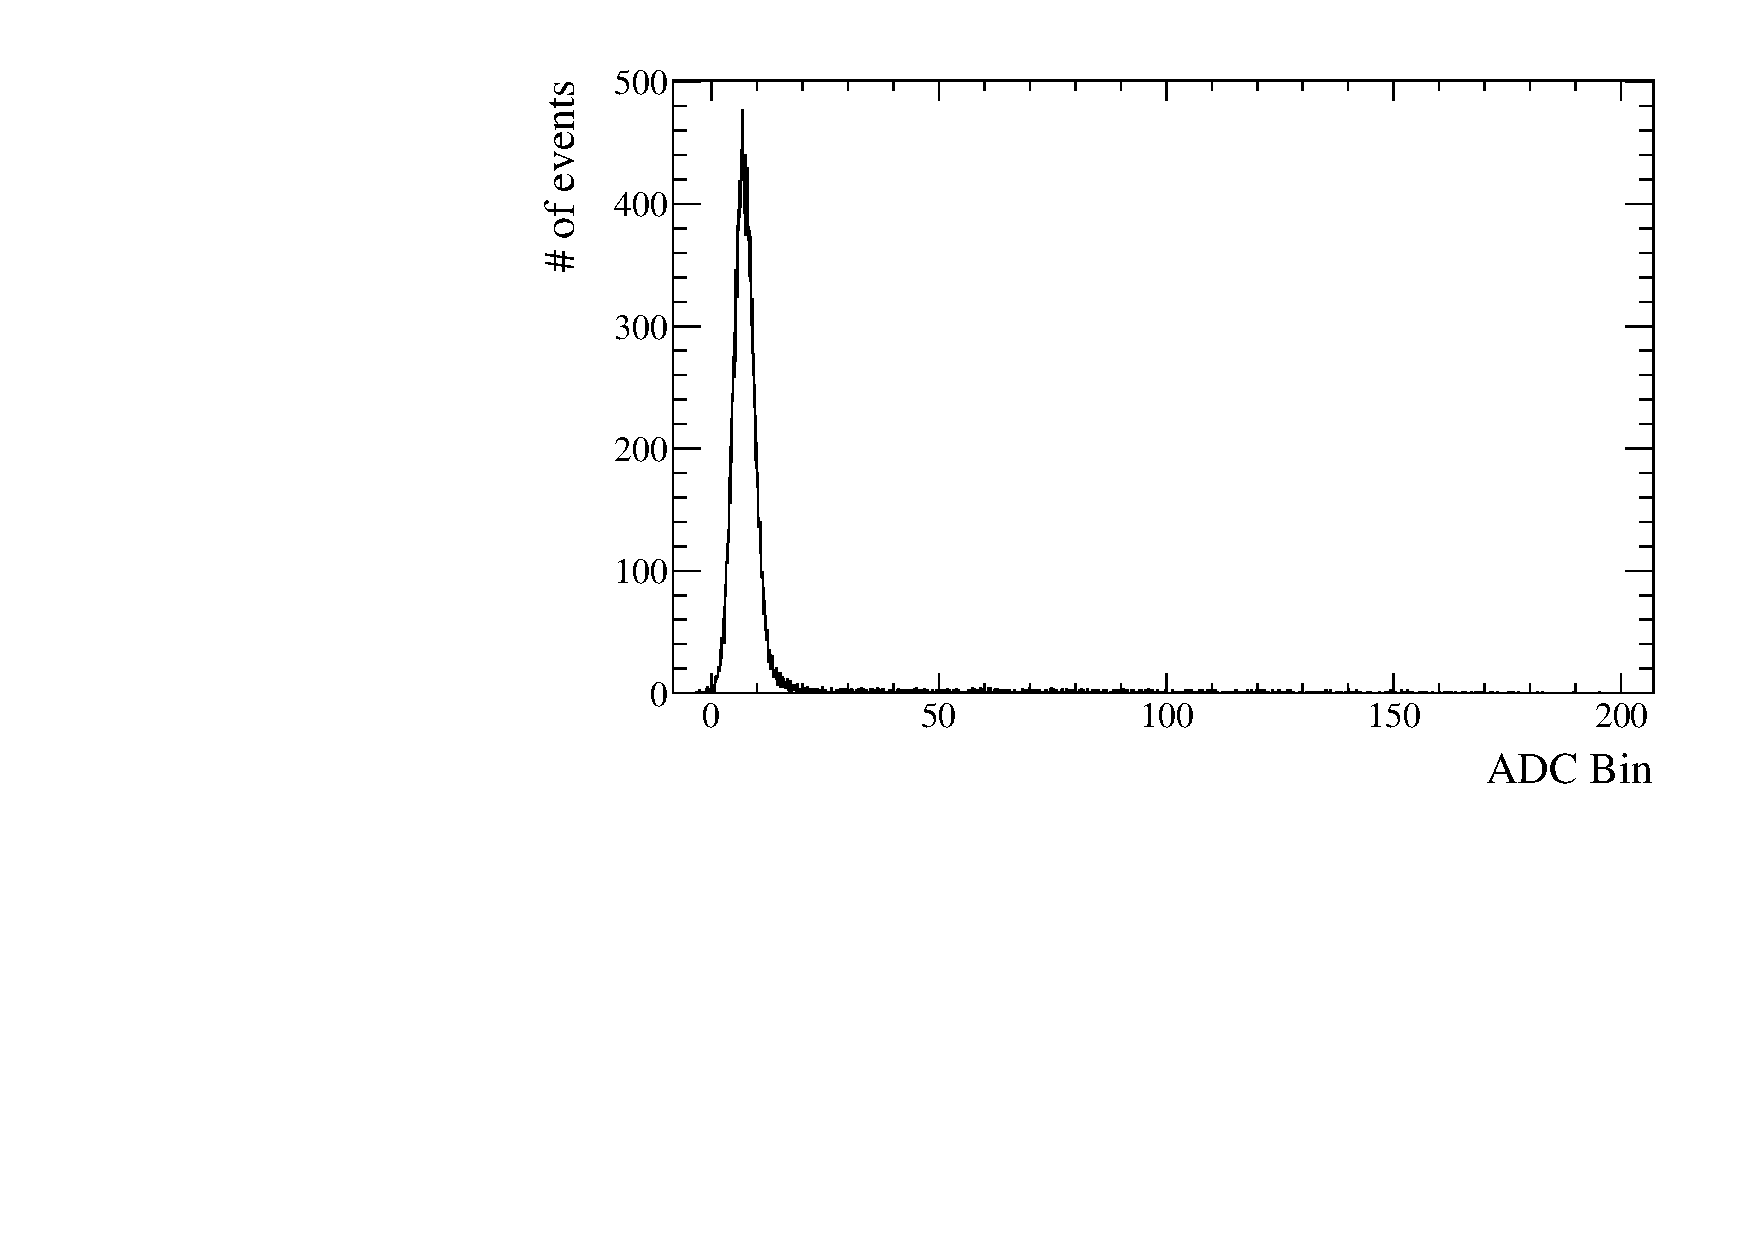
\includegraphics[width=100mm]{baselineitself.pdf}
\caption{Typical baseline value for a single channel.} \label{typicalbaseline}
\end{figure}

\begin{figure}[ht]
\centering
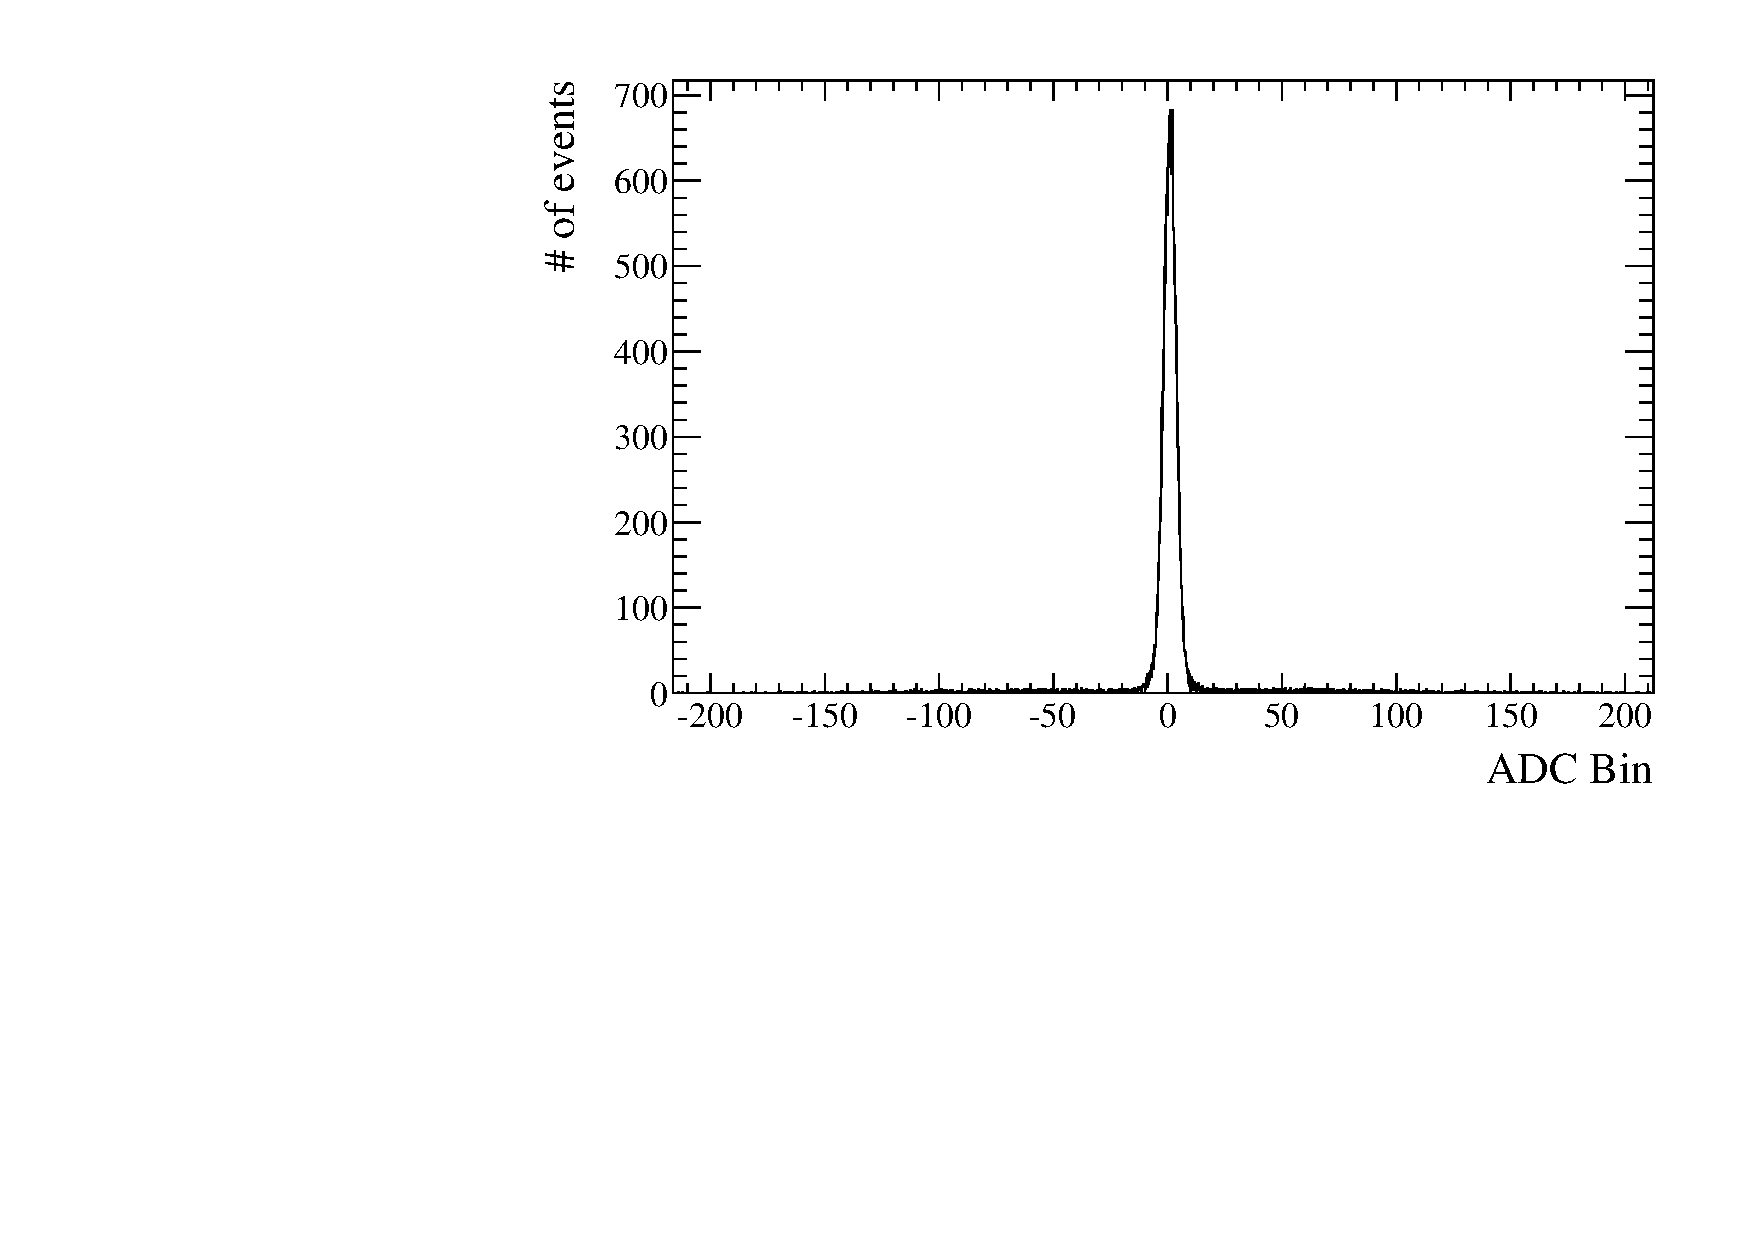
\includegraphics[width=100mm]{baselinedifference.pdf}
\caption{Difference between the baseline and the average of the post-signal window.} \label{baselinedifference}
\end{figure}


A baseline is defined as the average value of all the points in the first integration window (between the two red lines) that is 50ns wide. A typical baseline is shown in (Figure~\ref{typicalbaseline}) To check the baseline quality, its averaged value is compared agains the average of the post-signal window (between two blue lines). This difference is illustrated in (Figure~\ref{baselinedifference}). Events with this difference larger then $\sim$20 ADC bins are flagged as bad. This allows for the removal of the noise events or events with the bad baseline. Additionally, a comparison of the baseline with an average of a window at the very beginning of the waveform (between 10ns and 40ns, not shown because the figure is zoomed around the signal area) is used for general baseline quality check using the above criterion.


The integrated area is a measure of total charge that can be converted to the PE yield using the single PE calibration of the PMTs. This allows to describe the measured signals independent of the hardware differences between the channels.

The trigger information that is saved in the two additional FADC channels allows for the offline trigger requirements be used.

\subsection{Single Photo Electron Calibration}

A single PE calibration was conducted for both signal channels at the end of the test beam run. For it, the trigger is produced from the discriminator that follows the second amplifier for the T1 and T2 signals (separately for each, see Figure~\ref{experimentalsetup2}). The discriminator is set to $\sim$1/10\textsuperscript{th} of the single PE amplitude as to	allows for better PE signal detection efficiency than using random trigger. Additionally, this forces the PE signal to the signal window region of the FADC output for the simplified analysis and elimination of the partially captured signals. Note that a PE signal is much narrower and lower in amplitude/area then the beam signals that are typically many PEs that arrive with time disctibution, thus a smaller integration widnow is used to reduce noise for cleaner calibration (50ns instead of 300ns).

The signal area calibration is 168.0$\pm$1.2 ADC bins and 132.9$\pm$1.6 ADC bins for T1 and T2 respectively (the PE signal is summed within the window, so the unit of ADC bin is still used). A special care was taken to separately verify that this method yields the same calibration values as using the light-emmiting diode (LED) scheme. For that, calibration runs using the described above scheme and using the dim LED pulses were compared to each other. The LED light level is chosen such that only $\sim$1/10\textsuperscript{th} of the events has the single PE signal to insure that these are the single photon detection responces.


\subsection{Light Yield Analysis}


\subsubsection{Data selection}

\subsubsection{Energy deposition}

{
\renewcommand{\arraystretch}{1.2}
\begin{table}[htbp]
	\centering
		\caption{Energy Deposition in Samples}
		\label{tab:EnergyDepositionInSamples}
		\begin{tabular}{cccc}
		\hline \hline
		Beam Energy & Sample & T1 Energy & T2 Energy \\
		(MeV) & ~ & Deposit (MeV) & Deposit (MeV) \\ [0.5ex] \hline
		~ & Water, WbLS & 70 & 113 \\
    \raisebox{1.5ex}{210} & LS & 59 & 124 \\
    ~ & Water, WbLS & 39 & 42 \\
    \raisebox{1.5ex}{475} & LS & 34 & 36 \\
    ~ & Water, WbLS & 28 & 28 \\
    \raisebox{1.5ex}{2000} & LS & 24 & 24 \\
		[1ex] \hline
		\end{tabular}
\end{table}
}

\subsubsection{Light Yield Results}


\subsection{Systematics}

\subsubsection{Calibration Stability}

 \section{Conclusion}


%% References
%%
%% Following citation commands can be used in the body text:
%% Usage of \cite is as follows:
%%   \cite{key}          ==>>  [#]
%%   \cite[chap. 2]{key} ==>>  [#, chap. 2]
%%   \citet{key}         ==>>  Author [#]

%% References with bibTeX database:

\bibliographystyle{model1-num-names}
%%\bibliography{<your-bib-database>}

%% Authors are advised to submit their bibtex database files. They are
%% requested to list a bibtex style file in the manuscript if they do
%% not want to use model1-num-names.bst.

 %%References without bibTeX database:

 \begin{thebibliography}{00}

%% \bibitem must have the following form:
%%   \bibitem{key}...
%%
\bibitem{superKkinematik} M. Fechner et.al. (The Super-Kamiokande Collaboration),`Kinematic reconstruction of atmospheric neutrino events in a large water Cherenkov detector with proton identification', Phys. Rev. D 79 (2009) 112010, arXiv:0901.1645
\bibitem{hamamatsu} Hamamatsu Photonics, 314-5 Shimokanzo, Toyooka-village, Iwatagun, Shizuoka-ken, 438-0193 Japan; http://www.hamamatsu.com
\bibitem{caen} CAEN (Costruzioni Apparecchiature Elettroniche Nucleari S.p.A.), Via della Vetraia 11, 55049 Viareggio, Province of Lucca, Italy, 0584 388398.
\bibitem{phillips} Phillips Scientific, 31 Industrial Ave. Suite 1, Mahwah, N.J.  07430



 \end{thebibliography}
%% The Appendices part is started with the command \appendix;
%% appendix sections are then done as normal sections
%% \appendix

\end{document}

%%
%% End of file `elsarticle-template-1-num.tex'.
